\documentclass[main.tex]{subfiles}
\begin{document}
% neue TOC:
% \begin{itemize}
%     \item DONE wie im konzept gesagt vergleichen wir algorithmen um \$FRAGE zu beantworten
%     \item DONE zunächst definieren wir, wie und woran wir die performanz der algos vergleichen
%     \begin{itemize}
%         \item DONE Wir werden die performanz an 3 metriken messen: P,R,F1 (siehe BG section)
%     \end{itemize}
%     \item wie im konzept festgestellt, sind die pdas nicht vergleichbar. daher haben wir 2 verschiedene datensätze rausgesucht und oder erstellt:
%     \begin{itemize}
%         \item 2D 3D S: statisch, direkt ganze wolke da
%         \item FIN: dynamisch, inkrementell aufbauend
%     \end{itemize}
%     \item wir führen experimente auf beiden datensätzen durch 
%     \item im anschluss werten wir die ergebnisse aus und evaluieren inwiefern die algorithmen echtzeitfähig sind
% \end{itemize}

\chapter{Evaluation}

In diesem kapitel werden zuvor ausgewählte algorithmen einheitlich verglichen und die resultierenden ergebnisse ausgewertet.
\section{Protocol}
% \begin{itemize}
%     \item was wir zeigen wollen
%     \item daher vergleichen wir algorithmen
%     \item wie vergleichen wir, woran ziehen wir schlüsse? 
% \end{itemize}
This work aims to determine which plane detection algorithm is the most suitable for an AR/VR system. For this decision, we uniformly compare the algorithms selected in
Chapter~\ref{chap:Concept}. We split the comparison into two experiments conducted on different datasets: the 2D-3D-S and the
self-created FIN dataset. Since both data sets are fundamentally different, we will perform the experiments and the analysis separately and then compare the results.
First, we present the metrics used for comparison, followed by an outline of the used configurations of parameters for each experiment.
% In this work, we perform a uniform comparison of plane detection algorithms. This comparison aims to evaluate the real-time plane 
% detection on off-the-shelf hardware through the selection of the best algorithm.
% In the following subsection, we present the metrics used for the evaluation.
% We conduct experiments on both datasets and compare the results of both experiments with respect to the real-time applicability of the
% algorithms. Particularly interesting are the differences resulting from the temporal component.
% Finally, by evaluating the results of both experiments, we determine the most suitable plane detection algorithm for real-time, indoor environments. 

\subsection{Metrics}
To quantify the accuracy of the plane detection algorithms, we use the detected planes and the created ground truth to calculate the three following
performance metrics: Precision, Recall, and the F1-score. The procedure of calculation is taken from~\cite[Section~4]{Araújo_Oliveira_2020} and detailed
in Section~\ref{sec:metrics}.

\textcolor{red}{hier noch mehr ins detail gehen? (antwort) \underline{\hspace{2cm}}}

In addition to the accuracy of an algorithm, we precisely measure the calculation time by splitting the calculation into pre-processing, plane
detection, and post-processing. The Pre-processing step could include the estimation of normal vectors or the spatial subdivision
of a point cloud with an octree. If present, post-processing steps are primarily used for the refinement of the detected planes.

\subsection{Parameterization of Algorithms}
Da die Datensätze verschieden viel noise haben müssen die algorithmen in der hinsicht angepasst werden.
Es werden die parametrisierungen der Algorithmen im bezug auf die zwei experimente umrissen.
Dabei werden wir im fogenden die parametrisierung des 2D-3D-S datensatzes als den default ansehen.
Alle Abweichungen von diesem Default, die für den FIN Datensatz nötig waren, wurden empirisch ermittelt.


\subsubsection{RSPD}
% FIXME maybe test RSPD with other params and ggf rerun
\begin{table}[H]
    \centering
    \begin{tabular}{c|ccccc}
        Parameter      & $l_O$ & $\varepsilon$ & $\theta_{outlier}$ & $k$ \\ \hline
        2D-3D-S values & 10    & 30            & 25\%               & 30  \\
        FIN value      & 10    & 30            & 25                 & 30
    \end{tabular}%
    \caption{Parameter configuration of RSPD used for the experiments.}
    \label{tab:rspd-param}
\end{table}

\paragraph{2D-3D-S}
For the 2D-3D-S experiment, we took the given and all the included parameters. These parameters include the maximum octree level $l_O$,
the mini

\paragraph{FIN}
hier kommt ne begründung warum die parameter von RSPD beim FIN experiment so gewählt wurden.

\subsubsection{OPS}
The parameter configurations for both experiments are shown in Table~\ref{tab:ops-param}.
We use a sampling rate $\alpha_s$ of 3\% and 30 nearest-neighbors for the estimation of normal vectors since the dataset has an insignificant
amount of noise. Additionally, we use a distance threshold $\theta_h$ of 0.05(m) because the planes inside the dataset are very thin.
Furthermore, we set the inlier threshold $\theta_N$ to 100 and leave the probability $p$ for adaptively determining RANSAC iterations at $0.99$, as proposed
in the paper~\cite[Section~4A]{Sun_Mordohai_2019}.

\textcolor{red}{ja, die parameter werden im background \textit{sicherlich} erklärt}
\begin{table}[H]
    \centering
    \begin{tabular}{c|ccccc}
        Parameter      & $\alpha_s$ & $KNN$       & $\theta_{h}$  & $\theta_{N}$ & $p$  \\ \hline
        2D-3D-S values & 0.03       & 30          & 0.05          & 100          & 0.99 \\
        FIN values     & 0.03       & \textbf{90} & \textbf{0.35} & 100          & 0.99
    \end{tabular}%
    \caption{Parameter configuration of OPS used for the experiments.}
    \label{tab:ops-param}
\end{table}

\paragraph{2D-3D-S}
\paragraph{FIN}

\subsubsection{3D-KHT}
The parameter configuration is determined empirically and shown in Table~\ref{tab:3dkht-param}. We use an accumulator discretization of 30 and 200 for $\phi$ and $\rho$, respectively.
Using an octree starting level $s_{level}$ of 2 for the planarity check seemed to yield the best results. \citeauthor{Limberger_Oliveira_2015}\cite{Limberger_Oliveira_2015} propose
a minimum of 30 samples per cluster, however, we use $0.2\%$ of the total point cloud due to the wide ranges of point cloud sizes in the dataset.
Lastly, we use an $s_\beta$ value of 6, as proposed in the paper. In contrast, using a $s_\alpha$ value of 18 seemed to yield better results than the proposed 25.
% FIXME im background sicher gehen dass ich die erklärt habe
\begin{table}[H]
    \centering
    \begin{tabular}{c|ccccccc}
        Parameter      & $\phi_{num}$ & $\rho_{num}$ & $s_{level}$ & $s_{ps}$ & $d_{max}$    & $s_\alpha$ & $s_\beta$ \\ \hline
        2D-3D-S values & 30           & 200          & 2           & 0.002    & 0.08         & 18         & 6         \\
        FIN values     & 30           & \textbf{100} & 2           & 0.002    & \textbf{0.1} & \textbf{8} & 6
    \end{tabular}%
    \caption{Parameter configuration of 3D-KHT used for the experiments.}
    \label{tab:3dkht-param}
\end{table}
\paragraph{2D-3D-S}
\paragraph{FIN}

\subsubsection{OBRG}
We use the parameter configuration we empirically determined during the implementation. They are shown in Table~\ref{tab:obrg-param}.
Due to the low level of noise, we can assign a very low tolerance to $\theta_{res}$ and $\theta_d$. Similarly, we assign a high
planarity threshold value of $\theta_p = 90\%$.
\begin{table}[H]
    \centering
    \begin{tabular}{c|cccccc}
        Parameter      & $l_{max}$ & $\theta_{res}$ & $\theta_{d}$ & $\theta_{ang}$ & $\theta_M$ & $\theta_p$ \\ \hline
        2D-3D-S values & 5         & 0.08           & 0.08         & 0.18           & 5000       & 0.9        \\
        FIN values     & 5         & 0.22           & 0.2          & 0.2            & 5000       & 0.7
    \end{tabular}
    \caption{Parameter configuration of OBRG used for the experiments.}
    \label{tab:obrg-param}
\end{table}
\paragraph{2D-3D-S}
\paragraph{FIN}


% \paragraph{OPS}
% Because of the higher level of noise, we increase the size of the neighborhood and the parameter relating to plane thickness, $\theta_h$.
% The changes are shown in bold in Table~\ref{tab:fin-ops}.

% \begin{table}[H]
%     \centering
%     \begin{tabular}{c|ccccc}
%         Parameter & $\alpha_s$ & $KNN$       & $\theta_{h}$  & $\theta_{N}$ & $p$  \\ \hline
%         Value     & 0.03       & \textbf{90} & \textbf{0.35} & 100          & 0.99
%     \end{tabular}%
%     \caption{Parameter configuration of OPS used for the FIN experiment.}
%     \label{tab:fin-ops}
% \end{table}

% \paragraph{3D-KHT}
% The parameter configuration for 3D-KHT is once again determined empirically.
% For this experiment, we modify the values of $\rho_{num}$, $d_{max}$ and $s_\alpha$ to accommodate for the higher levels of noise.
% While reducing the $\rho$ discretization should decrease the accuracy, we find it to work better in a high-noise environment like the FIN dataset.
% We increase $d_{max}$ and decrease $s_\alpha$ to allow for slightly thicker, e.g. noisier, planes to be detected. The changes are reported in bold in
% Table~\ref{tab:fin-3dkht}.

% % FIXME im background sicher gehen dass ich die erklärt habe
% \begin{table}[H]
%     \centering
%     \begin{tabular}{c|ccccccc}
%         Parameter & $\phi_{num}$ & $\rho_{num}$ & $s_{level}$ & $s_{ps}$ & $d_{max}$    & $s_\alpha$ & $s_\beta$ \\ \hline
%         Value     & 30           & \textbf{100} & 2           & 0.002    & \textbf{0.1} & \textbf{8} & 6
%     \end{tabular}%
%     \caption{Parameter configuration of 3D-KHT used for the FIN experiment.}
%     \label{tab:fin-3dkht}
% \end{table}

% \paragraph{OBRG}
% The modifications to the configuration were determined empirically and are shown in Table~\ref{tab:fin-obrg}.
% Due to higher levels of noise, and thus, thicker walls, we increase the residual threshold $\theta_{res}$, the distance
% threshold $\theta_d$, and the angular divergence threshold $\theta_{ang}$. A planarity threshold, in this work referred to as $\theta_p$,
% should be chosen between 70\% and 90\% depending on the noise level~\cite[Section~3.4]{Vo_Truong-Hong_Laefer_Bertolotto_2015}. Therefore,
% we reduce this threshold to 70\%.
% \begin{table}[H]
%     \centering
%     \begin{tabular}{c|cccccc}
%         Parameter & $l_{max}$ & $\theta_{res}$ & $\theta_{d}$ & $\theta_{ang}$ & $\theta_M$ & $\theta_p$ \\ \hline
%         Value     & 5         & 0.22           & 0.2          & 0.2            & 5000       & 0.7
%     \end{tabular}
%     \caption{Parameter configuration of OBRG used for the FIN experiment.}
%     \label{tab:fin-obrg}
% \end{table}

\section{Results}
This section deals with the results of the experiments. The individual results of both experiments are presented and analyzed.
% FIXME RE-RUN OBRG and RSPD 
\subsection{Results 2D-3D-S Experiments}
% \begin{table}[H]
%     \centering
%     \begin{tabular}{c|ccccll}
%         3D-KHT Results  & Precision      & Recall         & F1-Score       \\ \hline
%         Auditorium      & 0.679          & 0.651          & 0.664          \\
%         Conference Room & 0.716          & 0.657          & 0.674          \\
%         Copy Room       & 0.584          & 0.714          & 0.642          \\
%         Hallway         & 0.734          & 0.700          & 0.707          \\
%         Lobby           & 0.650          & 0.625          & 0.637          \\
%         Lounge          & 0.449          & 0.447          & 0.429          \\
%         Office          & 0.673          & 0.719          & 0.683          \\
%         Open Space      & \textbf{0.813} & \textbf{0.857} & \textbf{0.834} \\
%         Pantry          & 0.758          & 0.782          & 0.770          \\
%         Storage         & 0.624          & 0.732          & 0.664          \\
%         WC              & 0.755          & 0.712          & 0.721          \\\hline
%         TOTAL           & 0.676          & 0.691          & 0.675
%     \end{tabular}
%     \caption[2D-3D-S 3DKHT Results]{Average results of 3D-KHT. The results of all areas are grouped by scene type and averaged. The bottom row shows the total average
%         over the entire dataset. Highlighted in bold are the best results.}
%     \label{tab:2s3ds-res-3dkht}
% \end{table}

% \begin{table}[H]
%     \centering
%     \begin{tabular}{c|ccccll}
%         OPS Results     & Precision      & Recall         & F1-Score       \\ \hline
%         Auditorium      & \textbf{0.957} & 0.835          & \textbf{0.890} \\
%         Conference Room & 0.942          & 0.617          & 0.699          \\
%         Copy Room       & 0.935          & 0.680          & 0.787          \\
%         Hallway         & 0.874          & 0.620          & 0.681          \\
%         Lobby           & 0.814          & 0.634          & 0.708          \\
%         Lounge          & 0.861          & 0.799          & 0.826          \\
%         Office          & 0.878          & 0.621          & 0.682          \\
%         Open Space      & 0.868          & \textbf{0.903} & 0.885          \\
%         Pantry          & 0.882          & 0.682          & 0.769          \\
%         Storage         & 0.898          & 0.506          & 0.596          \\
%         WC              & 0.945          & 0.642          & 0.715          \\ \hline
%         TOTAL           & 0.896          & 0.685          & 0.749
%     \end{tabular}
%     \caption[2D-3D-S OPS Results]{Average results of OPS. The results of all areas are grouped by scene type and averaged. The bottom row shows the total average
%         over the entire dataset. Highlighted in bold are the best results.}
%     \label{tab:2s3ds-res-ops}
% \end{table}

\begin{table}[H]
    \centering
    \begin{tabular}{c|cccccc}
        Results 2D-3D-S & Precision & Recall & F1     & $t_{pre}$ & $t_{calc}$ & $t_{post}$ \\ \hline
        RSPD            & 87.0\%    & 90.3\% & 88.3\% & 0.08      & 1.46       & /          \\
        OPS             & 89.6\%    & 68.5\% & 75.0\% & 1.14      & 21.23      & $<0.1$     \\
        3DKHT           & 67.6\%    & 69.1\% & 67.5\% & 2.62      & 1.61       & /          \\
        OBRG            & 83.2\%    & 62.8\% & 69.5\% & 39.85     & 47.25      & 2.89
    \end{tabular}
    \caption[Overall 2D-3D-S Results]{Average results of each algorithm over the 2D-3D-S dataset. The right half of the columns shows the average time spent in
        pre-processing ($t_{pre}$), the average time spent in the plane detection itself ($t_{calc}$), and the average time spent in post-processing steps ($t_{post}$).
        Note, that the absence of post-processing steps is denoted as "/".}
    \label{tab:res-3d2ds-total}
\end{table}

\textcolor{red}{das hier stimmt jetzt obv nicht mehr da neue ergebnisse}

The results of each algorithm on the 2D-3D-S dataset are shown in Table~\ref{tab:res-3d2ds-total}.
RSPD produces the overall best results with an average of 85\% precision, 89\% recall and an F1-score of 86\%, as well as an average of 0.9 seconds of calculation time.
The only other algorithm that achieves similar calculation times is 3D-KHT, which takes 0.91 seconds on average. Considering our definition of \textit{real-time} in Section~\ref{sec:realtime},
RSPD and 3D-KHT are able to perform plane detecion in real-time. Still, 3D-KHT produces the worst overall accuracy results with an average precision of 75\%, recall of 43\%, and an F1-score of 53\%.

With an average of about 17 seconds(OPS) and about 44 seconds(OBRG), both algorithms do not achieve real-time plane detection (see Table~\ref{tab:res-3d2ds-total}).


\begin{figure}[H]
    \centering
    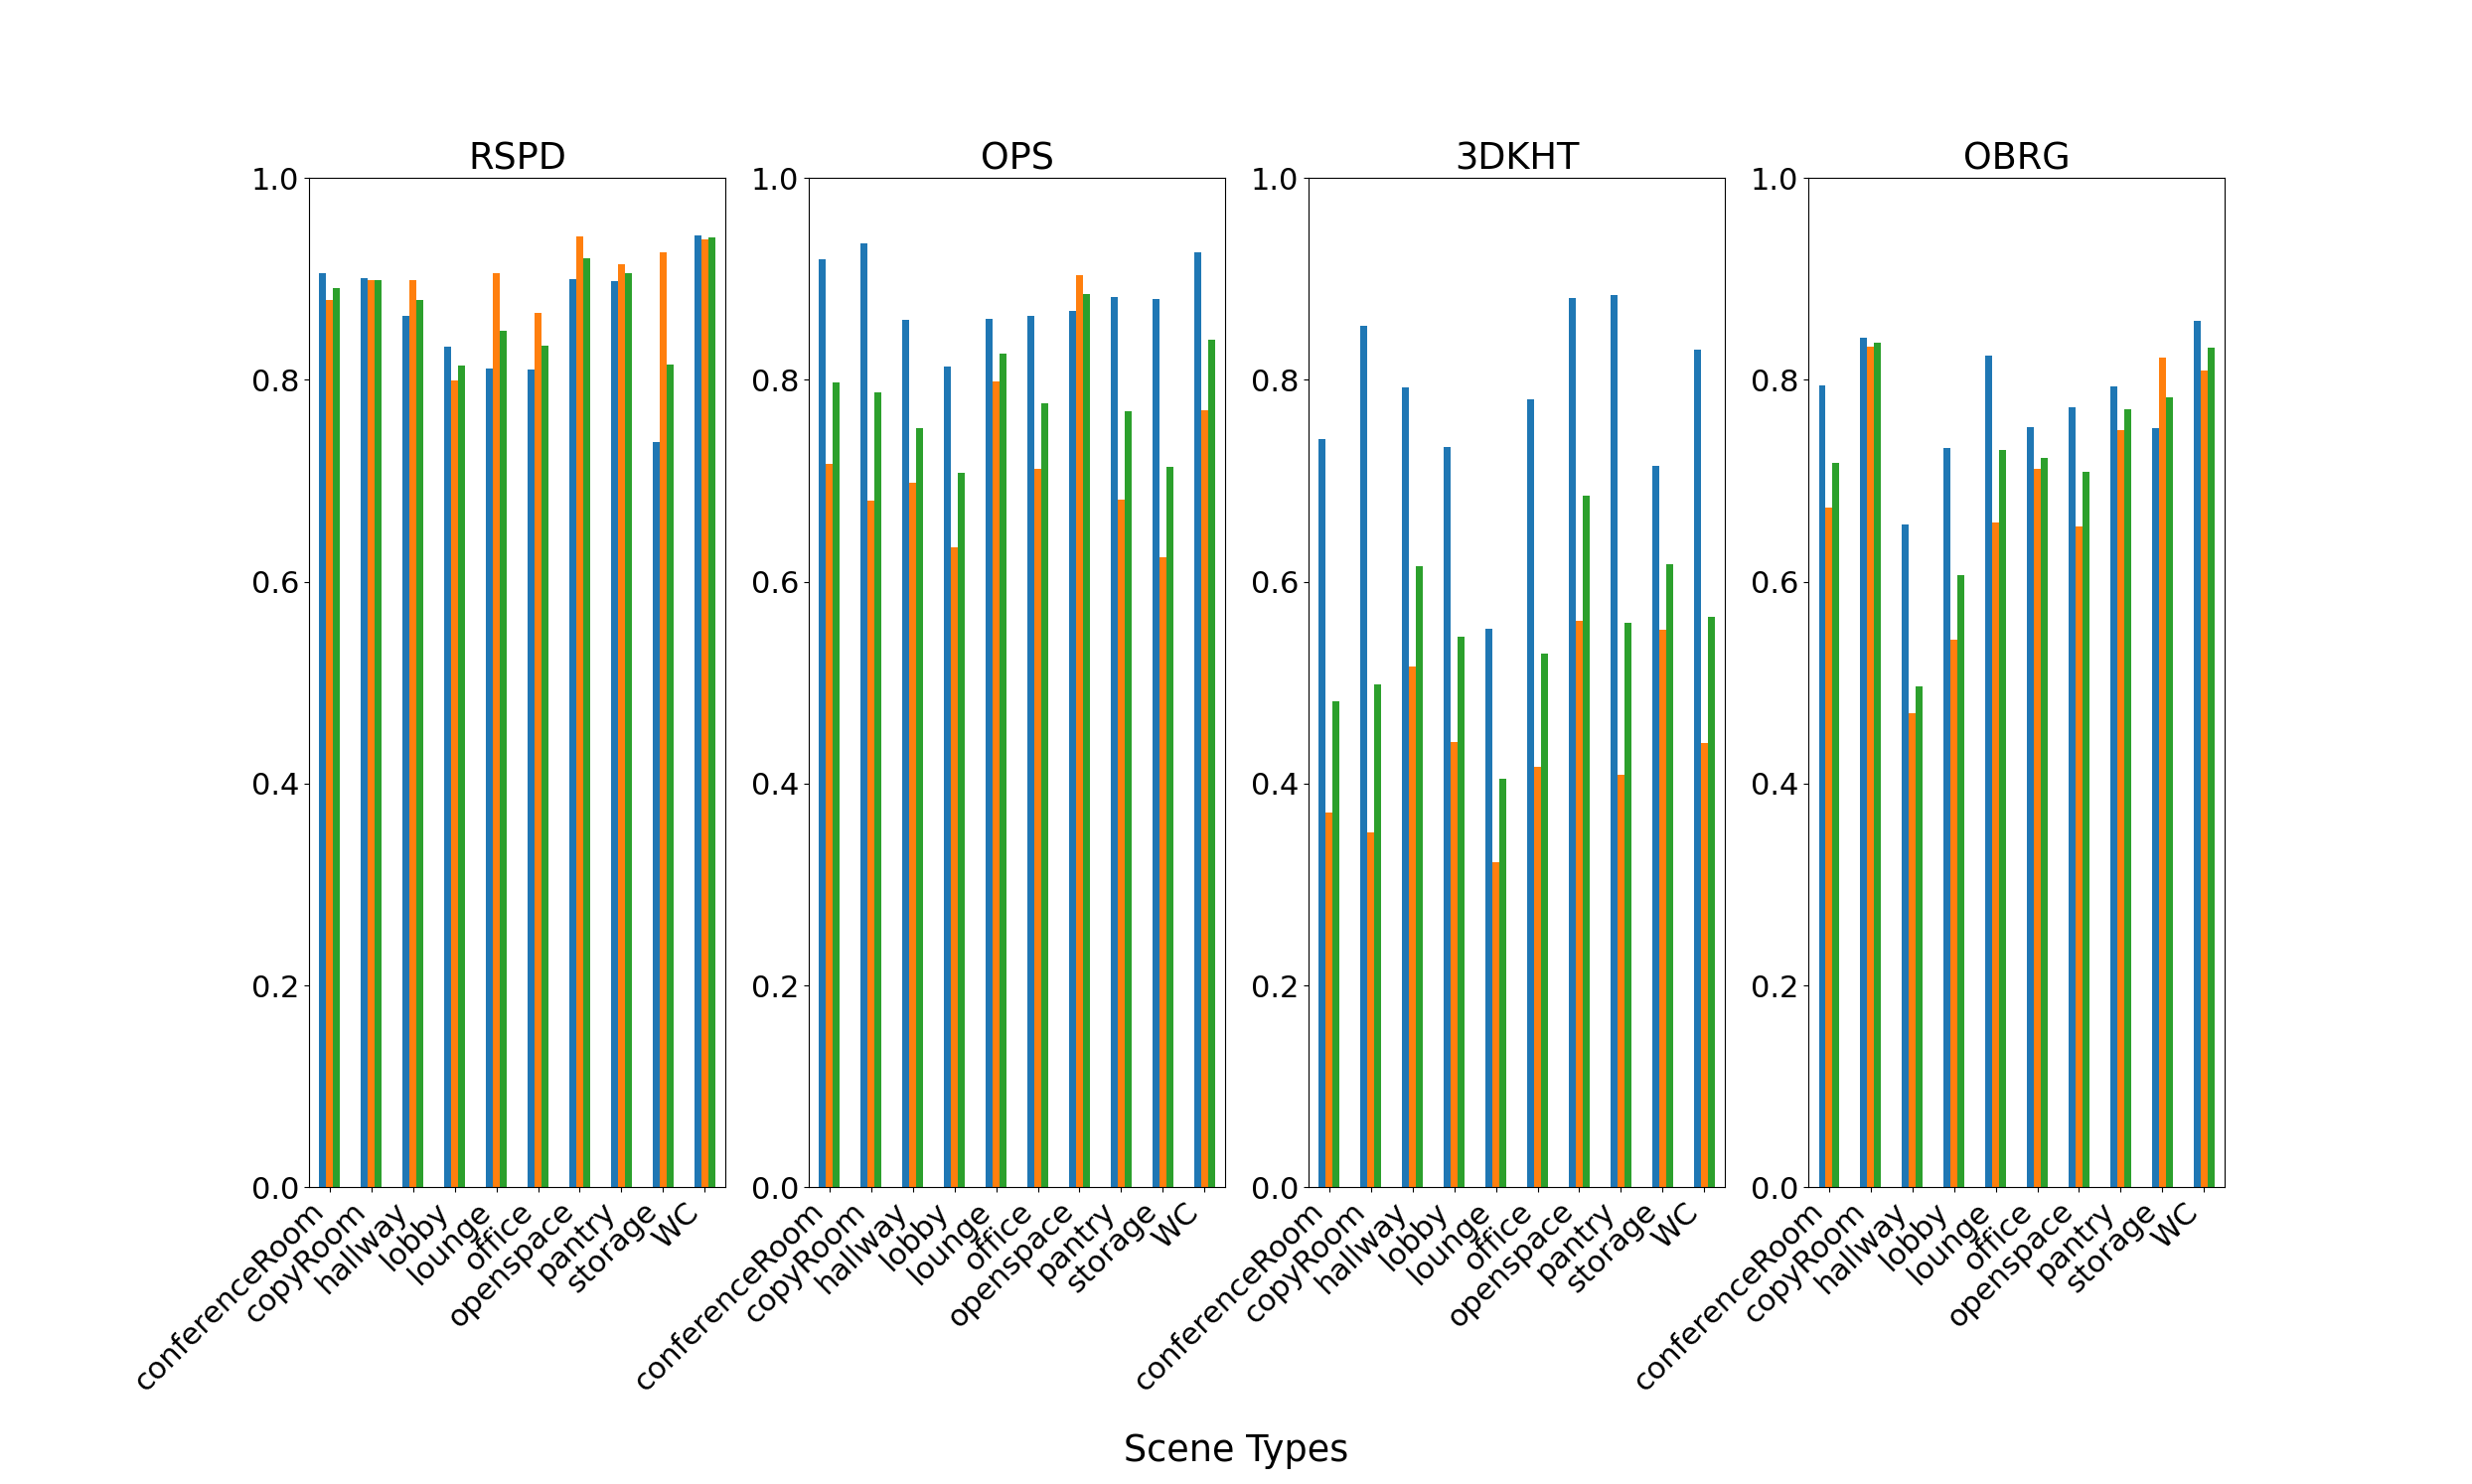
\includegraphics[width=\textwidth]{images/accuracy_total.png}
    \caption[Accuracy Results 2D-3D-S]{Average Accuracy for each scene type. The Precision
        is colored blue, recall is orange and the F1-score is green.}
    \label{fig:stanfordaccuracy}
\end{figure}

\begin{figure}[H]
    \centering
    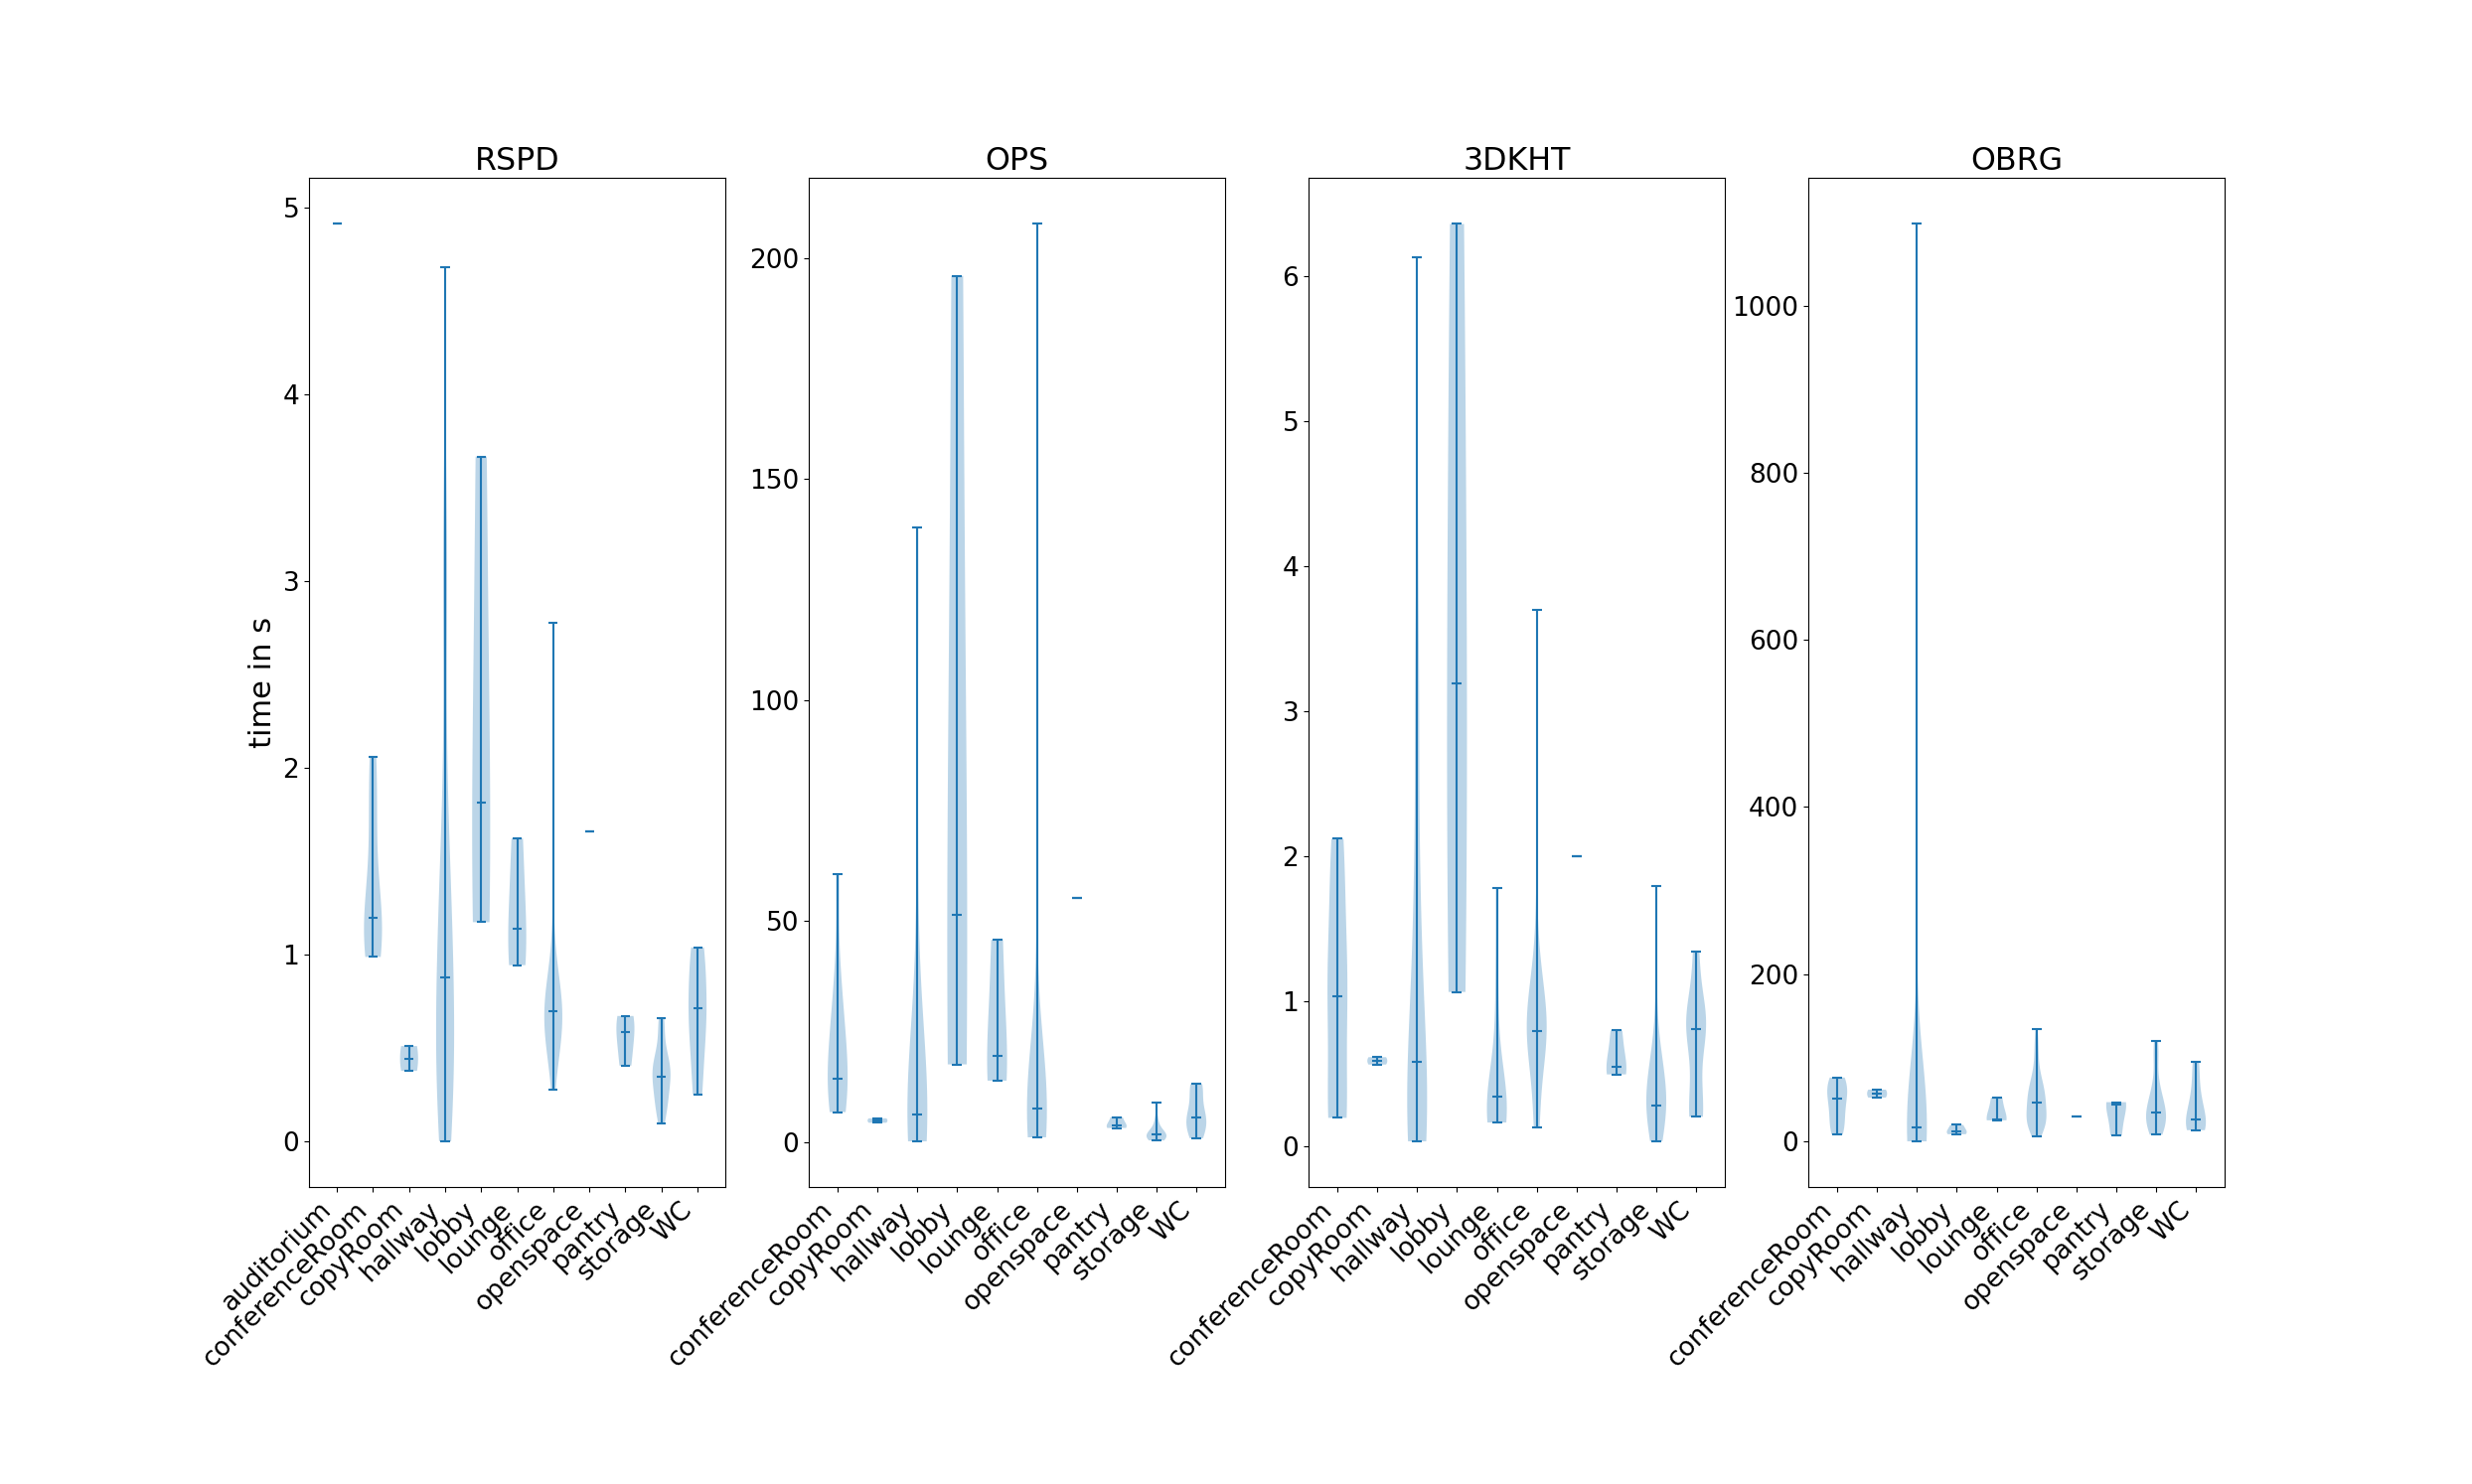
\includegraphics[width=15 cm]{images/times_violin.png}
    \caption[Time Results 2D-3D-S]{Times per scene type. The lowest tick denotes the minimum time, the highest
        denotes the maximum time spent in the calculation. The middle tick shows the mean time.
        Note, that the plots
        do not share the same y-axis.}
    \label{fig:violintime}
\end{figure}

\subsection{Results Real-Life Experiments}
\textit{So far:}

\begin{figure}[]
    \centering
    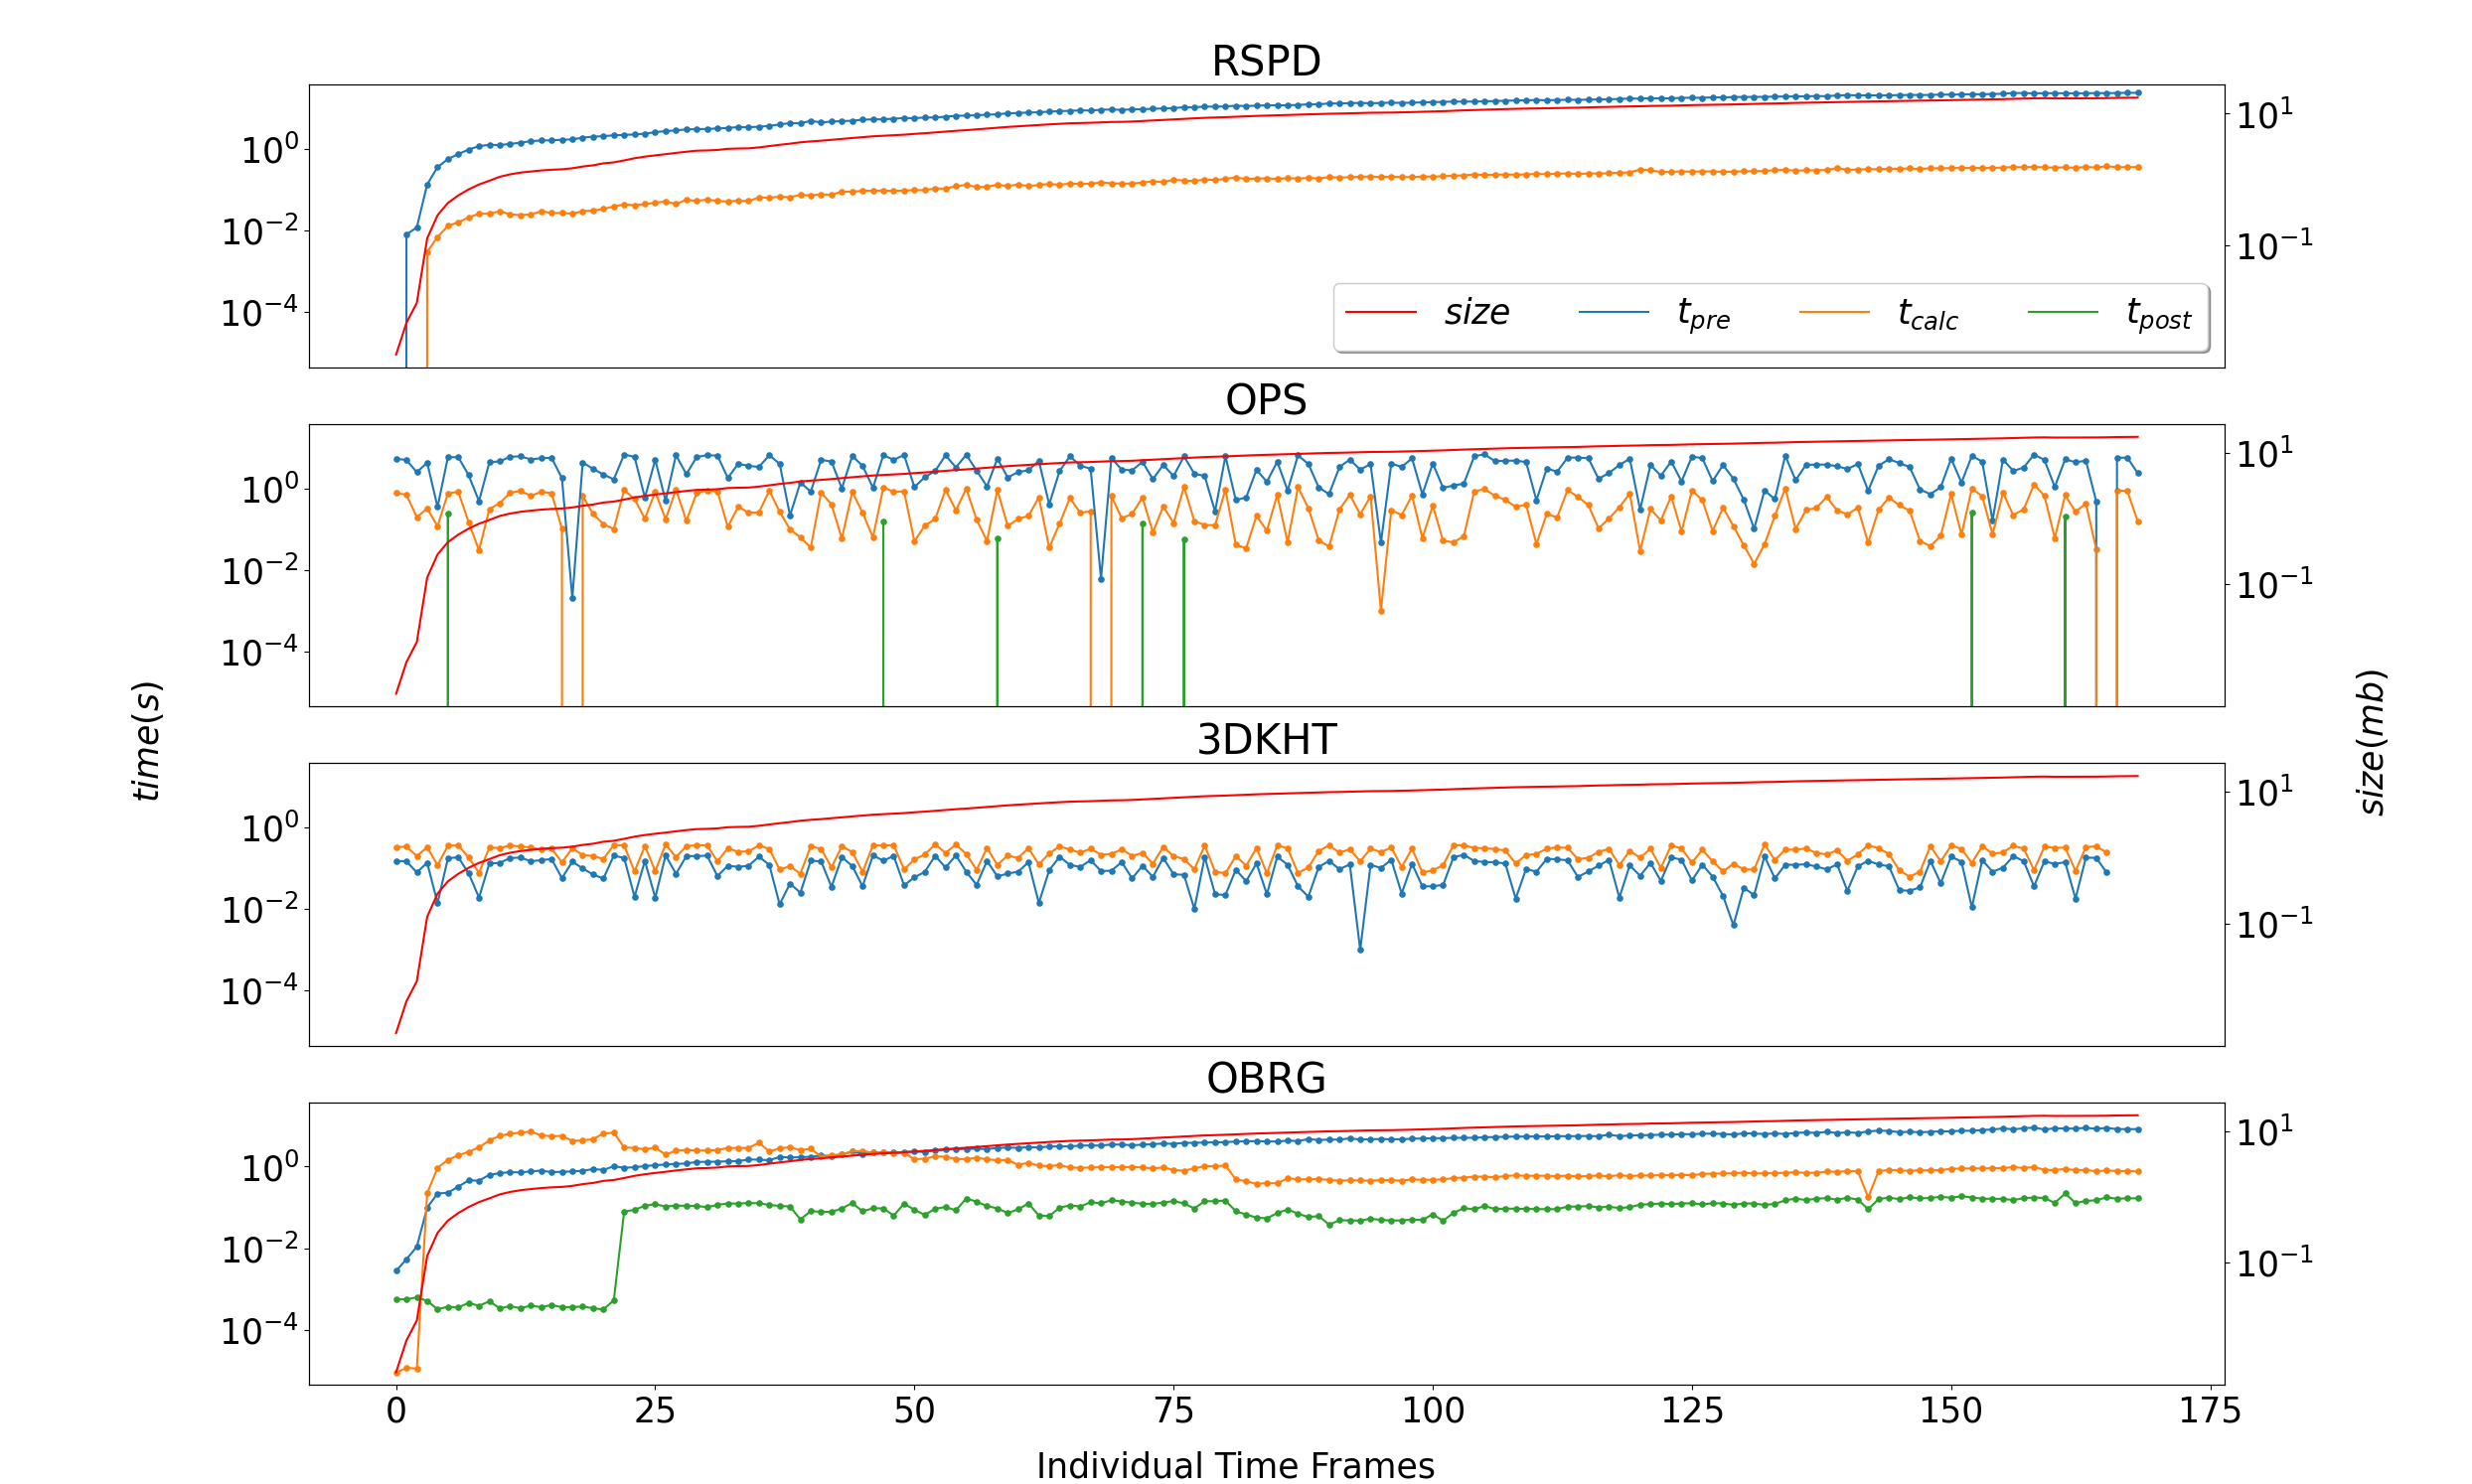
\includegraphics[width=\textwidth]{images/dyn_time-hallway.png}
    \caption[Time Results Hallway]{Calculation times(blue) of the hallway scene and cloud size(red) of each time step.}
    \label{fig:dynhallway}
\end{figure}

The calculation times of all algorithms except OBRG seem to be proportional to the size of the point cloud.
% TODO similar figure for 2D-3D-S
The quality of plane detection, however, decreases dramatically in comparison to the Stanford Datasets. RSPD is the only dataset that
is able to detect planes. %(see Figure~\ref{fig:}). 

% FIXME RERUN RSPD, OPS for time
% FIXME RERUN OBRG on all except office, conferenceroom 
\begin{table}[H]
    \centering
    \begin{tabular}{c|cccccc}
        Results FIN & Precision & Recall & F1-Score & $t_{pre}$ & $t_{calc}$ & $t_{post}$ \\ \hline
        RSPD        & 0.51      & 0.56   & 0.54     &           &            & /          \\
        OPS         & 0.69      & 0.29   & 0.39     & 1.14      & 21.23      & $<0.1$     \\
        3DKHT       & 0.49      & 0.44   & 0.46     & 0.14      & 0.29       & /          \\
        OBRG        & 0.11      & 0.06   & 0.08     & 3.08      & 7.08       & 2.89
    \end{tabular}
    \caption[Overall 2D-3D-S Results]{Average results of each algorithm over the FIN dataset. The right half of the columns shows the average time spent in
        pre-processing ($t_{pre}$), the average time spent in the plane detection itself ($t_{calc}$), and the average time spent in post-processing steps ($t_{post}$).
        Note, that the absence of post-processing steps is denoted as "/".}
    \label{tab:res-fin-total}
\end{table}

\textcolor{red}{Average zeiten bei einem wachsenden datensatz sind sinnlos.. oder? da finde ich macht die korrelation zwischen größe 
der punktwolke und dauer der berechnung mehr sinn}


\begin{table}[]
    \centering
    \begin{tabular}{c|cccccc}
               & Precision & Recall & F1-Score \\ \hline
        RSPD   & 38.9\%    & 50.4\% & 43.8\%   \\
        OPS    & 47.1\%    & 30.5\% & 36.8\%   \\
        3D-KHT & 32.0\%    & 32.4\% & 31.9\%   \\
        OBRG   & 50.8\%    & 34.5\% & 40.6\%
    \end{tabular}%
    \caption{Average Results for the auditorium scene of the FIN dataset.}
    \label{tab:res-fin-audi}
\end{table}

\begin{table}[]
    \centering
    \begin{tabular}{c|cccccc}
               & Precision & Recall & F1-Score & $t_{pre}$             & $t_{calc}$            & $t_{post}$            \\ \hline
        RSPD   & 58.2\%    & 63.2\% & 60.5\%   & \textcolor{red}{todo} & \textcolor{red}{todo} & \textcolor{red}{todo} \\
        OPS    & 69.9\%    & 28.8\% & 39.9\%   & \textcolor{red}{todo} & \textcolor{red}{todo} & \textcolor{red}{todo} \\
        3D-KHT & 47.4\%    & 45.9\% & 46.2\%   & 0.21                  & 0.42                  & /                     \\
        OBRG   & 38.8\%    & 28.5\% & 32.7\%   & 8.13                  & 117.72                & 0.65
    \end{tabular}%
    \caption{Average Results for the conferenceRoom scene of the FIN dataset.}
    \label{tab:res-fin-conf}
\end{table}

\begin{table}[]
    \centering
    \begin{tabular}{c|ccc}
               & Precision          & Recall             & F1-Score           \\ \hline
        RSPD   & 0.50               & 0.51               & 0.51               \\
        OPS    & 0.87               & 0.20               & 0.32               \\
        3D-KHT & 0.57               & 0.44               & 0.49               \\
        OBRG   & \textcolor{red}{0} & \textcolor{red}{0} & \textcolor{red}{0}
    \end{tabular}%
    \caption{Average Results for the hallway scene of the FIN dataset.}
    \label{tab:res-fin-hall}
\end{table}

\begin{table}[]
    \centering
    \begin{tabular}{c|ccc}
               & Precision & Recall & F1-Score \\ \hline
        RSPD   & 71.1\%    & 69.9\% & 70.4\%   \\
        OPS    & 74.7\%    & 37.1\% & 49.2\%   \\
        3D-KHT & 62.3\%    & 54.9\% & 58.2\%   \\
        OBRG   & 46.8\%    & 27.3\% & 34.0\%
    \end{tabular}
    \caption{Average Results for the office scene of the FIN dataset.}
    \label{tab:res-fin-off}
\end{table}

\subsection{Summary Results}
% NOTE 3DKHT kann keine löcher oder non-rectangular ebenen basteln!
This section combines the preceding results of both experiments.
RSPD is the only algorithm that produces comparable results to the Stanford experiment in the dynamic experiment.
The remaining algorithms cannot reliably detect planes in an incrementally growing environment inheriting varying degrees of noise.

The reason for RSPD's dominance is likely caused by the inherent robustness against noise, as described in Section~

Die ergebnisse der beiden experimente unterscheiden sich in folgendem punkt. Dazu sei gesagt, dass die experimente folgende übereinstimmungen haben.
Das lässt sich so erklären. Alternative gründe davon könnten diese hier sein.

Ich denke RSPD ragt heraus, da hier besonders auf noise resistenz geachtet wurde. % TODO verweis auf diverse noise tests im BG


\end{document}